% Hướng dẫn sử dụng Kriky, cho giáo viên và học sinh.
%
% Build: .\dev.ps1 user-guide   (latexmk -xelatex). Luật viết: rules.md.

\documentclass[11pt,a4paper,oneside]{book}

% Toàn bộ trang trí của hướng dẫn sử dụng: phông, màu, bìa, trang phần, tiêu đề, ô mẹo, nút, ảnh
% có số. Nạp bởi user-guide.tex. Luật viết và bảng các lệnh ở rules.md.
%
% Khác báo cáo một cách có chủ ý: đây là tài liệu cho giáo viên và học sinh thật, đọc trên màn hình,
% nên nó mang nhận diện của Kriky (phông, màu của app và chú dế) thay cho khuôn đồ án.
%
% BẮT BUỘC XeLaTeX (`.\dev.ps1 user-guide`). Mọi phông nạp thẳng từ tệp .ttf trong fonts/, nên máy
% build không cần cài phông nào.

% ---------------------------------------------------------------- Phông và ngôn ngữ
\usepackage{fontspec}
\usepackage{polyglossia}
\setmainlanguage{vietnamese}

% Be Vietnam Pro là phông của app (services/fe/index.html), giấy phép OFL ở fonts/OFL.txt.
% Scale 0.94: phông này rộng, 11pt của nó trông như 12pt.
% Bốn độ đậm, mỗi độ một series riêng: m (thường), mb (Medium, nhãn), b (SemiBold, \textbf),
% eb (Bold, tiêu đề lớn). Đặt Bold vào `b` thì BoldFont đè mất nó (review pha 2).
\setmainfont{BeVietnamPro}[
  Path           = fonts/,
  Extension      = .ttf,
  Scale          = 0.94,
  UprightFont    = *-Regular,
  ItalicFont     = *-Italic,
  BoldFont       = *-SemiBold,
  BoldItalicFont = *-BoldItalic,
  FontFace       = {mb}{n}{*-Medium},
  FontFace       = {eb}{n}{*-Bold},
]
\newcommand{\vua}{\fontseries{mb}\selectfont}     % Medium: nhãn, chữ trên nút
\newcommand{\datdam}{\fontseries{eb}\selectfont}  % Bold: tiêu đề lớn, số chương
\linespread{1.22}

\usepackage[a4paper,left=2.3cm,right=2.3cm,top=2.6cm,bottom=2.4cm,headsep=0.8cm,
  headheight=16pt]{geometry}
\setlength{\emergencystretch}{3em}
\tolerance=2000
\raggedbottom

% ---------------------------------------------------------------- Màu
% Màu của app lấy đúng mã trong services/fe/src/tokens.css; màu của chú dế lấy từ kriky-hero.png.
\usepackage[table]{xcolor}
\definecolor{sunken}{HTML}{F2F2EF}
\definecolor{ink}{HTML}{1A1F2B}
\definecolor{inkmuted}{HTML}{5B6472}
\definecolor{line}{HTML}{E3E5E2}
\definecolor{accent}{HTML}{2E4A7D}
\definecolor{accentsurface}{HTML}{EDF1F7}
\definecolor{correct}{HTML}{2F6B45}
\definecolor{correctsurface}{HTML}{EDF1EE}
\definecolor{incorrect}{HTML}{8C3A3A}
\definecolor{incorrectsurface}{HTML}{F7ECEC}
\definecolor{needshuman}{HTML}{8A5A22}
\definecolor{needshumansurface}{HTML}{F6EFE4}
\definecolor{processing}{HTML}{2F6F73}
\definecolor{processingsurface}{HTML}{E8F1F1}
% Chú dế.
\definecolor{krikyorange}{HTML}{E9740C}
\definecolor{krikyorangedeep}{HTML}{B65A0A}
\definecolor{krikyorangesoft}{HTML}{FDF1E2}
\definecolor{krikyyellow}{HTML}{FEC053}
\definecolor{krikyyellowsoft}{HTML}{FFF6E0}
\definecolor{krikygreen}{HTML}{6E8B2E}
\definecolor{krikygreensoft}{HTML}{EEF3E1}

% Màu của phần đang đọc: xanh cho giáo viên, cam cho học sinh, xanh lá cho phần chung. Chỉ dùng để
% trang trí (trang phần, vạch tiêu đề, đầu trang, số trang); nút trong sách luôn mang màu nút của app.
\colorlet{phan}{krikygreen}
\colorlet{phansoft}{krikygreensoft}
\color{ink}

% ---------------------------------------------------------------- Gói chung
\usepackage{graphicx}
% Ảnh của chú dế đọc thẳng từ app, nên đổi mặt Kriky ở app là sách đổi theo.
\graphicspath{{screenshots/}{figures/}{../../services/fe/public/}}
\usepackage{tikz}
\usetikzlibrary{calc,positioning,shadows.blur}
\usepackage[most]{tcolorbox}
\usepackage{fontawesome5}
\usepackage{booktabs}
\usepackage{array}
\usepackage{xltabular}
\usepackage{enumitem}
\usepackage{etoolbox}            % \ifstrequal của \trangphan
\usepackage{needspace}
\usepackage{titlesec}
\usepackage{titletoc}
\usepackage{fancyhdr}
\usepackage[font=small,labelfont={color=inkmuted},textfont={color=inkmuted}]{caption}
\usepackage[unicode,colorlinks=true,linkcolor=accent,urlcolor=accent]{hyperref}
\hypersetup{pdftitle={Hướng dẫn sử dụng Kriky},pdflang={vi}}

\setlength{\parindent}{0pt}
\setlength{\parskip}{0.55em}
\setlist{itemsep=0.15em,topsep=0.3em}
\newcolumntype{L}[1]{>{\raggedright\arraybackslash}p{#1}}
\newcolumntype{Y}{>{\raggedright\arraybackslash}X}
\renewcommand{\arraystretch}{1.35}

% ---------------------------------------------------------------- Chữ trên màn hình
% \nut{Duyệt đề}: một nút của app, vẽ thành viên thuốc màu nút của app, để người đọc nhận ra đúng
% thứ mình đang tìm trên màn hình. tcbox chứ không \tikz: \tikz trong nhãn danh sách hỏng với
% polyglossia.
\newtcbox{\nutbox}{on line, colback=accentsurface, colframe=accent!55, coltext=accent,
  boxrule=0.5pt, arc=3.5pt, left=3.5pt, right=3.5pt, top=0.6pt, bottom=0.6pt, boxsep=0pt,
  fontupper=\vua\small}
\newcommand{\nut}[1]{\nutbox{\strut#1}}
% \nhan{Tên lớp}: tên một ô, một nhãn hay một dòng chữ trên app (không bấm được).
% \leavevmode trước \color: đứng đầu một ô bảng, \color mở đoạn mới và đẩy ô xuống một dòng.
\newcommand{\nhan}[1]{\leavevmode{\vua\color{ink}“#1”}}
% \go{...}: chữ ngắn người dùng gõ vào, nguyên văn. Cùng phông với app, trên nền xám như ô nhập.
\newtcbox{\gobox}{on line, colback=sunken, colframe=line, boxrule=0.5pt, arc=2.5pt, left=3pt,
  right=3pt, top=0.5pt, bottom=0.5pt, boxsep=0pt}
\newcommand{\go}[1]{\gobox{\strut#1}}
% \begin{loinhan} ... \end{loinhan}: một câu nhắn dài gửi Kriky, xuống dòng được, như bong bóng
% chat của giáo viên (nằm bên phải).
\newtcolorbox{loinhan}{enhanced, breakable, colback=accentsurface, colframe=accentsurface,
  boxrule=0pt, arc=8pt, left=0.8em, right=0.8em, top=0.4em, bottom=0.4em,
  width=0.82\linewidth, flush right, before skip=0.4em, after skip=0.6em}
% Chữ còn chờ người dùng điền (địa chỉ lab…). Cố ý chói, để không lọt ra bản gửi đi.
\newcommand{\chocandien}[1]{\leavevmode{\color{incorrect}\vua[cần điền: #1]}}

% ---------------------------------------------------------------- Số bước
% Cùng một chấm cam trên ảnh và trong danh sách bước: số ① trên ảnh là bước ① bên dưới. Cam đậm
% (krikyorangedeep) để số trắng đủ tương phản.
\newtcbox{\sobox}{on line, colback=krikyorangedeep, colframe=krikyorangedeep, coltext=white,
  boxrule=0pt, circular arc, left=0pt, right=0pt, top=0pt, bottom=0pt, boxsep=0pt,
  fontupper=\datdam\footnotesize, width=1.4em, height=1.4em, valign=center, halign=center,
  tcbox width=forced center}
\newcommand{\sobuoc}[1]{\raisebox{-0.3em}{\sobox{#1}}}
\newlist{buoc}{enumerate}{1}
\setlist[buoc]{label=\sobuoc{\arabic*}, leftmargin=2.2em, labelsep=0.6em, itemsep=0.35em,
  topsep=0.4em}

% ---------------------------------------------------------------- Ảnh chụp có số
% \anh[bề rộng]{tệp}{lớp phủ}. Trong lớp phủ, toạ độ tính theo ảnh: x từ trái 0 → phải 1, y từ
% trên 0 → dưới 1 (đúng chiều đọc trên màn hình), nên đo vị trí trên ảnh xong là chép vào được.
%   \diem{2}{0.31}{0.12}           chấm số 2 có tâm tại (31%, 12%): đặt CẠNH chỗ bấm, không đè lên
%   \khung{0.05}{0.10}{0.40}{0.20} viền cam quanh một vùng (trái, trên, phải, dưới)
% Ảnh cao quá 0,55 trang thì co theo chiều cao, để không tràn trang.
\tikzset{
  sotren/.style={circle, fill=krikyorangedeep, draw=white, line width=1.2pt, text=white,
    font=\datdam\footnotesize, inner sep=0pt, minimum size=1.45em,
    blur shadow={shadow blur steps=4, shadow xshift=0.3pt, shadow yshift=-0.4pt,
      shadow opacity=35}},
}
\newcommand{\diem}[3]{\node[sotren] at (#2,{1-#3}) {#1};}
\newcommand{\khung}[4]{\draw[krikyorangedeep, line width=1.4pt, rounded corners=3pt]
  (#1,{1-#2}) rectangle (#3,{1-#4});}
% Ảnh chưa chụp thì in một ô xám chói thay vì làm hỏng cả bản build: một chỗ trống phải thấy được
% trên trang, không được lặng lẽ biến mất.
\newcommand{\anh}[3][\dimexpr\linewidth-2pt\relax]{%
  \IfFileExists{screenshots/#2.png}{\anhco[#1]{#2}{#3}}{%
    \par\smallskip\begin{center}\fcolorbox{incorrect}{sunken}{\parbox[c][3cm][c]{0.8\linewidth}{%
      \centering\color{incorrect}\vua ảnh chưa chụp: #2}}\end{center}\smallskip}}
\newcommand{\anhco}[3][]{%
  \par\smallskip
  \begin{center}
  \begin{tikzpicture}
    \node[inner sep=0, anchor=south west, blur shadow={shadow blur steps=6, shadow xshift=0pt,
      shadow yshift=-1pt, shadow opacity=18}] (img) at (0,0)
      {\includegraphics[width=#1,height=0.55\textheight,keepaspectratio]{#2}};
    \draw[line, line width=0.6pt] (img.south west) rectangle (img.north east);
    \begin{scope}[x={(img.south east)}, y={(img.north west)}]
      #3
    \end{scope}
  \end{tikzpicture}
  \end{center}
  \smallskip}

% ---------------------------------------------------------------- Các ô
% Ba ô, ba màu khác hẳn nhau: vàng (lời khuyên của Kriky), hổ phách (cần để ý), đỏ (khi hỏng).
% Chữ trong ô cùng cỡ thân bài: một câu cảnh báo không được nhỏ hơn câu thường.
\tcbset{ougo/.style={enhanced, breakable, boxrule=0pt, arc=6pt, left=3.6em, right=0.9em,
  top=0.6em, bottom=0.6em, before skip=0.7em, after skip=0.7em}}
\newtcolorbox{machnhobox}{ougo, colback=krikyyellowsoft, colframe=krikyyellowsoft,
  borderline west={3pt}{0pt}{krikyyellow},
  overlay unbroken and first={\node[anchor=north west, inner sep=0] at
    ([xshift=0.7em,yshift=-0.5em]frame.north west)
    {
\includegraphics[width=2.3em]{kriky-face.png}};}}
\newcommand{\machnho}[1]{\begin{machnhobox}{\vua\color{krikyorangedeep}Kriky mách nhỏ\par}
  \vspace{0.1em}#1\end{machnhobox}}

\newtcolorbox{luuybox}{ougo, colback=needshumansurface, colframe=needshumansurface,
  borderline west={3pt}{0pt}{needshuman},
  overlay unbroken and first={\node[anchor=north west, text=needshuman] at
    ([xshift=0.95em,yshift=-0.7em]frame.north west) {\LARGE\faExclamationTriangle};}}
\newcommand{\luuy}[1]{\begin{luuybox}{\datdam\color{needshuman}Lưu ý\par}\vspace{0.1em}#1%
  \end{luuybox}}

\newtcolorbox{neuloibox}{ougo, colback=incorrectsurface, colframe=incorrectsurface,
  borderline west={3pt}{0pt}{incorrect},
  overlay unbroken and first={\node[anchor=north west, text=incorrect] at
    ([xshift=1em,yshift=-0.7em]frame.north west) {\LARGE\faTools};}}
\newcommand{\neuloi}[1]{\begin{neuloibox}{\datdam\color{incorrect}Nếu gặp lỗi\par}\vspace{0.1em}#1%
  \end{neuloibox}}

% \xong{...}: dấu hiệu việc đã xong. Một dòng xanh, dính với danh sách bước ngay trên nó.
\newcommand{\xong}[1]{\par\nopagebreak\smallskip\leavevmode{\color{correct}\faCheckCircle\enspace\vua Xong
  khi:}\enspace#1\par}

% ---------------------------------------------------------------- Tiêu đề
\newcommand{\phanhientai}{}
\titleformat{\chapter}[display]{\color{ink}}
  {\tikz\node[fill=phan, text=white, rounded corners=8pt, minimum width=3.1em,
     minimum height=3.1em, font=\datdam\huge]{\thechapter};}
  {0.6em}
  {\datdam\fontsize{24}{30}\selectfont}
  [\vspace{0.35em}{\color{phan}\titlerule[1.2pt]}]
\titleformat{name=\chapter,numberless}[display]{\color{ink}}{}{0pt}
  {\datdam\fontsize{24}{30}\selectfont}[\vspace{0.35em}{\color{phan}\titlerule[1.2pt]}]
\titlespacing*{\chapter}{0pt}{-1.2em}{1.4em}

% Mỗi "việc" là một \section: tiêu đề có vạch màu của phần bên trái.
\titleformat{\section}[block]{\color{ink}\vua\Large}
  {}{0pt}{{\color{phan}\rule[-0.2em]{3.5pt}{1.15em}}\hspace{0.6em}}
\titlespacing*{\section}{0pt}{1.6em}{0.5em}
\titleformat{\subsection}[block]{\color{phan}\vua\large}{}{0pt}{}
\titlespacing*{\subsection}{0pt}{1.1em}{0.3em}
\setcounter{secnumdepth}{0}
% Mục lục chỉ tới chương: người đọc tìm chương của mình, rồi lật tới việc cần làm.
\setcounter{tocdepth}{0}
% Một việc mở đầu sát đáy trang thì tiêu đề nằm một trang, ảnh và các bước nằm trang sau: thà sang
% trang mới ngay từ tiêu đề.
\newcommand{\viec}[1]{\needspace{0.3\textheight}\section{#1}}

% ---------------------------------------------------------------- Mục lục
% Mục lục in màu chữ thường, không màu link; dòng phần mang màu của chính phần ấy (ghi vào toc).
\titlecontents{part}[0pt]{\addvspace{1.2em}\datdam\large}{}{}{\hfill\contentspage}[\addvspace{0.3em}]
\titlecontents{chapter}[2.4em]{\addvspace{0.45em}\vua}
  {\contentslabel[\thecontentslabel]{2.4em}}{}{\titlerule*[0.6pc]{.}\contentspage}
\titlecontents{section}[2.4em]{\small\color{inkmuted}}{}{}{\titlerule*[0.6pc]{.}\contentspage}
\newcommand{\mucluc}{\begingroup\hypersetup{linkcolor=ink}\tableofcontents\endgroup}

% ---------------------------------------------------------------- Đầu và chân trang
\newtcbox{\trangbox}{on line, colback=phansoft, colframe=phansoft, coltext=phan, boxrule=0pt,
  arc=6pt, left=7pt, right=7pt, top=2pt, bottom=2pt, boxsep=0pt, fontupper=\vua\small}
\pagestyle{fancy}
\fancyhf{}
\renewcommand{\headrulewidth}{0pt}
\fancyhead[L]{\small\color{inkmuted}\raisebox{-0.3em}{
\includegraphics[height=1.3em]{kriky-face.png}}%
  \enspace Hướng dẫn sử dụng Kriky}
\fancyhead[R]{\small\color{phan}\vua\phanhientai}
\fancyfoot[C]{\trangbox{\thepage}}
\fancypagestyle{plain}{\fancyhf{}\fancyfoot[C]{\trangbox{\thepage}}}

% ---------------------------------------------------------------- Trang phần
% \trangphan{gv|hs}{Phần I}{Dành cho thầy cô}{Lời dẫn một câu}{Các chương, mỗi chương một \item}
% Sang trang, đổi màu của phần, rồi in một trang màu với chú dế và danh sách chương. Đổi màu nằm
% bên trong lệnh này, nên không có thứ tự ngầm nào để gọi sai.
\newcommand{\trangphan}[5]{%
  \cleardoublepage
  \ifstrequal{#1}{gv}{\colorlet{phan}{accent}\colorlet{phansoft}{accentsurface}%
    \renewcommand{\phanhientai}{Phần I · Giáo viên}}{}%
  \ifstrequal{#1}{hs}{\colorlet{phan}{krikyorangedeep}\colorlet{phansoft}{krikyorangesoft}%
    \renewcommand{\phanhientai}{Phần II · Học sinh}}{}%
  \thispagestyle{empty}
  \phantomsection
  \label{phan:#1}%
  \ifstrequal{#1}{gv}{\addcontentsline{toc}{part}{\texorpdfstring{\protect\color{accent}#2 \textendash{} #3}{#2 – #3}}}{}%
  \ifstrequal{#1}{hs}{\addcontentsline{toc}{part}{\texorpdfstring{\protect\color{krikyorangedeep}#2 \textendash{} #3}{#2 – #3}}}{}%
  \begin{tikzpicture}[remember picture, overlay]
    \fill[phan] (current page.south west) rectangle (current page.north east);
    \fill[white, opacity=0.06] ([xshift=-2cm,yshift=-3cm]current page.north east) circle (6cm);
    \fill[white, opacity=0.05] ([xshift=3cm,yshift=4cm]current page.south west) circle (5cm);
    \node[anchor=north west, text=white, font=\vua\Large, inner sep=0]
      (so) at ([xshift=2.3cm,yshift=-4.2cm]current page.north west) {#2};
    \node[anchor=north west, text=white, font=\datdam\fontsize{38}{44}\selectfont, inner sep=0,
      text width=15cm] (ten) at ([yshift=-0.5cm]so.south west) {#3};
    \node[anchor=north west, text=white, text width=9.5cm, font=\large, inner sep=0]
      (dan) at ([yshift=-0.7cm]ten.south west) {#4};
    \node[anchor=north west, text=white, text width=9.5cm, inner sep=0]
      at ([yshift=-1.4cm]dan.south west) {%
        {\vua TRONG PHẦN NÀY\par}\vspace{0.4em}
        \begin{itemize}[leftmargin=1.2em, label={\color{krikyyellow}\textbullet}, itemsep=0.25em]
          #5
        \end{itemize}};
    \node[anchor=south east, inner sep=0] at ([xshift=-1.6cm,yshift=2.2cm]current page.south east)
      {
\includegraphics[height=9.5cm]{kriky-hero.png}};
  \end{tikzpicture}
  \clearpage}

% Phần chung (đầu sách, tra nhanh): màu xanh lá, đầu trang không ghi phần.
\newcommand{\phanchung}{\cleardoublepage
  \colorlet{phan}{krikygreen}\colorlet{phansoft}{krikygreensoft}%
  \renewcommand{\phanhientai}{}}

% ---------------------------------------------------------------- Bìa
\newcommand{\biasach}{%
  \begin{titlepage}
  \begin{tikzpicture}[remember picture, overlay]
    \fill[krikyyellowsoft] (current page.south west) rectangle (current page.north east);
    % Vài vòng tròn nền, màu của chú dế.
    \fill[krikyyellow!45] ([xshift=-3.6cm,yshift=11.6cm]current page.south east) circle (7cm);
    \fill[krikygreen!20] ([xshift=2.6cm,yshift=-3.0cm]current page.north west) circle (1.1cm);
    \fill[krikyorange!60] ([xshift=4.4cm,yshift=-2.4cm]current page.north west) circle (0.22cm);
    % Chú dế đứng trên dải đáy.
    \node[anchor=south east, inner sep=0] at ([xshift=-1.4cm,yshift=3.05cm]current page.south east)
      {
\includegraphics[height=13.4cm]{kriky-hero.png}};
    % Tên sách.
    \node[anchor=north west, text width=9.5cm, align=left, inner sep=0]
      (ten) at ([xshift=2.3cm,yshift=-7.2cm]current page.north west) {%
        {\color{krikyorangedeep}\vua\large HƯỚNG DẪN SỬ DỤNG\par}
        \vspace{0.35cm}
        {\color{accent}\datdam\fontsize{64}{64}\selectfont Kriky\par}
        \vspace{0.45cm}
        {\color{ink}\fontsize{19}{25}\selectfont Trợ lý giúp thầy cô ra đề\\và giúp các em chữa bài\par}};
    % Hai lối vào.
    \node[anchor=north west, inner sep=0] at ([yshift=-1.6cm]ten.south west) {%
      \begin{tabular}{@{}l@{\enspace}l@{}}
        {\color{accent}\Large\faChalkboardTeacher} & {\vua\large Thầy cô}\enspace
          {\color{inkmuted}đọc Phần I} \\[0.5em]
        {\color{krikyorangedeep}\Large\faUserGraduate} & {\vua\large Học sinh}\enspace
          {\color{inkmuted}đọc Phần II} \\
      \end{tabular}};
    % Dải đáy.
    \fill[accent] (current page.south west) rectangle ([yshift=3.1cm]current page.south east);
    \node[anchor=west, text=white, font=\vua\large]
      at ([xshift=2.3cm,yshift=1.75cm]current page.south west) {Phiên bản \tenban};
    \node[anchor=west, text=white!80!accent]
      at ([xshift=2.3cm,yshift=1.05cm]current page.south west) {\ngaysach};
  \end{tikzpicture}
  \end{titlepage}
  % Bìa là trang 1, như trình xem PDF đếm: số in trên trang khớp số trang người đọc thấy.
  \setcounter{page}{2}}

% ---------------------------------------------------------------- Bảng tra
% \begin{bangtra}{L{5cm}Y}{Cột 1 & Cột 2} ... \end{bangtra}
% Ngắt qua trang được (xltabular), hàng đầu lặp lại ở trang sau. Nền xen kẽ bắt đầu từ hàng dữ
% liệu đầu tiên. Không cắt đệm hai đầu bằng @{}: nền màu tô cả phần đệm, cắt chữ mà không cắt
% nền thì nền tràn ra lề; và bỏ khe của booktabs quanh vạch để nền không hở.
\newenvironment{bangtra}[2]
  {\par\smallskip
   \setlength{\aboverulesep}{0pt}\setlength{\belowrulesep}{0pt}%
   \rowcolors{3}{white}{sunken}%
   \xltabular{\linewidth}{#1}
   \toprule \rowcolor{phansoft}#2 \\ \midrule \endfirsthead
   \toprule \rowcolor{phansoft}#2 \\ \midrule \endhead
   \bottomrule \endlastfoot}
  {\endxltabular\par\smallskip}
\newcommand{\dau}[1]{\leavevmode{\color{phan}\vua #1}}

% Những thứ đổi theo mỗi lần gửi sách: chỗ duy nhất phải sửa khi ra bản mới.
%
% \tenban phải khớp tên bản hiện ở góc trái dưới của app, cũng là tên hiện trên mọi ảnh chụp
% (rules.md, mục Ảnh chụp).
\newcommand{\tenban}{lab-2026.0.4}
\newcommand{\ngaysach}{Tháng 11 năm 2026}
% Hai địa chỉ của lab. Chưa điền thì sách in chữ đỏ [cần điền: …], để không lọt ra bản gửi đi.
\newcommand{\diachigiaovien}{\chocandien{địa chỉ trang giáo viên}}
\newcommand{\diachihocsinh}{\chocandien{địa chỉ trang học sinh}}


\begin{document}

% polyglossia gọi mục lục là "Mục lục" sẵn; đặt lại sau \begin{document} cho chắc, vì nó nạp nhãn
% lúc tài liệu bắt đầu (cùng lý do như report.tex).
\renewcommand{\contentsname}{Mục lục}

\biasach

\phanchung
\mucluc

% Đầu sách: đọc tài liệu này thế nào. Không đánh số, để Phần I bắt đầu từ Chương 1.

\chapter*{Đọc tài liệu này thế nào}
\addcontentsline{toc}{chapter}{Đọc tài liệu này thế nào}

Ai cũng nên đọc mục \emph{Làm quen với Kriky}. Sau đó, thầy cô và các em chỉ cần đọc phần của mình.

\begin{bangtra}{L{4.2cm}L{3.2cm}Y}{\dau{Bạn là} & \dau{Đọc} & \dau{Trong đó}}
  Giáo viên & Phần I, trang~\pageref{phan:gv} & Lập lớp, soạn đề cùng Kriky, phát hành, xem
  kết quả \\
  Học sinh & Phần II, trang~\pageref{phan:hs} & Đăng nhập, làm bài, hỏi Kriky câu sai, làm
  lại \\
  Ai cũng nên đọc & Làm quen, trang~\pageref{chuong:lam-quen} & Kriky là ai, cần chuẩn bị gì \\
\end{bangtra}

\section{Các ký hiệu trong sách}

\begin{bangtra}{L{4.6cm}Y}{\dau{Thấy trong sách} & \dau{Nghĩa là}}
  \nut{Duyệt đề} & Một nút trên màn hình. Bấm vào đó. \\
  \nhan{Tên lớp} & Một ô, một nhãn hay một dòng chữ trên màn hình. \\
  \go{12A} & Chữ gõ vào, đúng từng chữ. \\
  \sobuoc{1} & Một bước. Số trên ảnh khớp với số ở bước. \\
  \leavevmode{\color{correct}\faCheckCircle\enspace\vua Xong khi:} & Thấy điều này là việc đã xong. \\
  \leavevmode{\color{krikyorangedeep}\vua Viền cam trên ảnh} & Vùng cần để ý trên màn hình. \\
  Ô xanh nhạt lệch phải & Một câu mẫu để nhắn cho Kriky. \\
\end{bangtra}

\machnho{Ô vàng có mặt Kriky là mẹo để làm nhanh hơn.}

\luuy{Ô nâu là điều cần để ý, bỏ qua dễ mất công làm lại.}

\neuloi{Ô đỏ chỉ cách xử lý khi màn hình báo lỗi.}

% Đầu sách: làm quen với Kriky. Không đánh số.

\chapter*{Làm quen với Kriky}
\addcontentsline{toc}{chapter}{Làm quen với Kriky}
\label{chuong:lam-quen}

Kriky là trợ lý giúp thầy cô ra đề kiểm tra trắc nghiệm, và giúp các em hiểu những câu mình làm sai.
Thầy cô nhắn cho Kriky bằng câu bình thường; Kriky soạn đề, thầy cô xem và duyệt. Chỉ thầy cô mới phát
hành được đề cho học sinh.

\section{Một bài kiểm tra đi qua những bước nào}

Hình~\ref{fig:vong-doi} cho thấy một bài kiểm tra đi từ lúc soạn tới lúc xem kết quả. Số trong mỗi ô
là thứ tự; dòng nhỏ dưới ô là chương nói về bước ấy.

\begin{figure}[htbp]
  \centering
  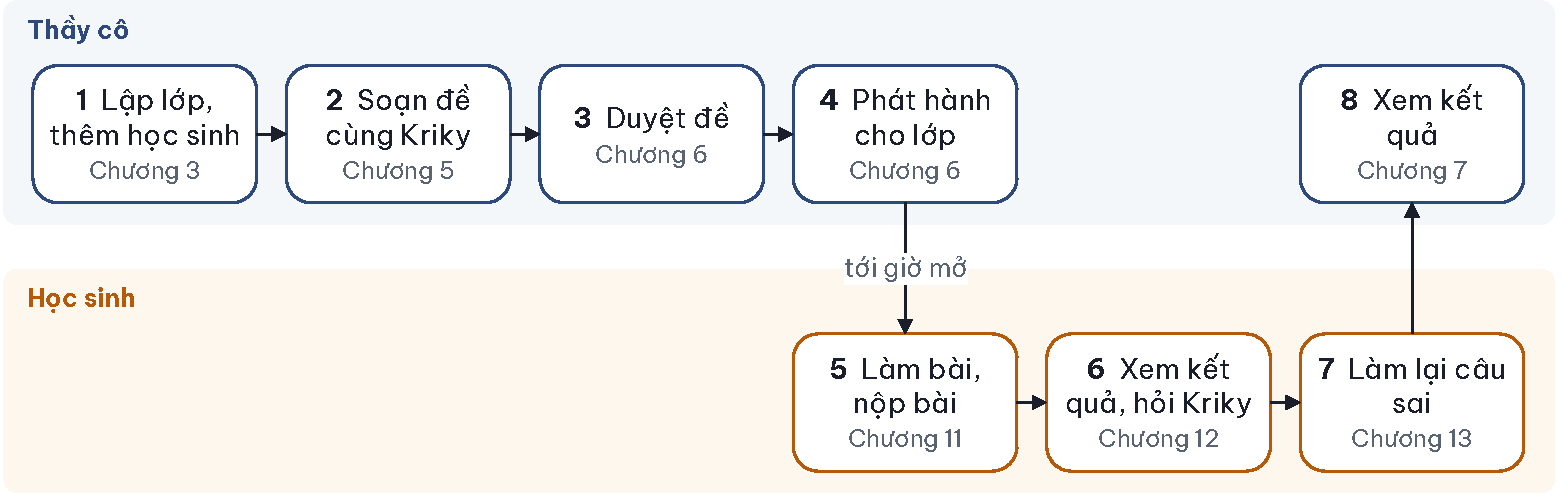
\includegraphics[width=\linewidth]{vong-doi-bai-kiem-tra.pdf}
  \caption[Vòng đời một bài kiểm tra]{Vòng đời một bài kiểm tra: thầy cô làm ở hàng trên, học sinh
    làm ở hàng dưới.}
  \label{fig:vong-doi}
\end{figure}

Bài làm có hai giai đoạn. Ở giai đoạn đầu, học sinh làm bài trong thời gian thầy cô đặt. Ở giai đoạn
hai, học sinh hỏi Kriky những câu mình sai, rồi làm một câu tương tự để gỡ điểm.

\section{Cần chuẩn bị gì}

\begin{bangtra}{L{3.6cm}Y}{\dau{Cần} & \dau{Chi tiết}}
  Máy tính & Màn hình máy tính hoặc laptop. Kriky được làm cho màn hình máy tính; trên điện thoại
  rất khó dùng. \\
  Trình duyệt & Chrome hoặc Edge bản mới. \\
  Địa chỉ trang giáo viên & \diachigiaovien \\
  Địa chỉ trang học sinh & \diachihocsinh \\
  Tài khoản giáo viên & Người quản lý Kriky của trường cấp (Chương~\ref{chuong:dang-nhap-gv}). \\
  Tài khoản học sinh & Thầy cô tạo cho cả lớp, rồi phát tên đăng nhập và mật khẩu cho từng em. \\
\end{bangtra}

\luuy{Thầy cô và các em dùng hai địa chỉ khác nhau. Học sinh vào nhầm trang giáo viên thì sẽ không đăng
nhập được bằng tên đăng nhập học sinh.}

\section{Bản Kriky đang dùng}

Góc trái dưới màn hình có tên bản, ví dụ \nhan{\tenban}. Sách này viết cho bản ấy. Khi cần báo lỗi,
bấm vào tên bản để chép lại (app không báo gì khi chép), rồi gửi kèm lời báo cho người quản lý Kriky
của trường.


% Phần I: giáo viên. Mở bằng trang phần, rồi từng chương ở 11–19.

\trangphan{gv}{Phần I}{Dành cho thầy cô}{Lập lớp, soạn đề cùng Kriky, phát hành cho học sinh và xem
kết quả.}{\item Đăng nhập \item Bản đồ màn hình \item Lớp và học sinh \item Tài liệu \item Soạn đề
cùng Kriky \item Duyệt và phát hành \item Theo dõi kết quả \item Ngân hàng câu hỏi \item Khi gặp
trục trặc}

\chapter{Đăng nhập}
\label{chuong:dang-nhap-gv}

Thầy cô mở địa chỉ trang giáo viên: \diachigiaovien. Tài khoản giáo viên do người quản lý Kriky của trường
cấp: thầy cô nhận số điện thoại hoặc email dùng để đăng nhập, cùng mật khẩu.

\viec{Đăng nhập}

\anh[0.62\linewidth]{T/01-dang-nhap}{
  \diem{1}{0.035}{0.24}
  \diem{2}{0.035}{0.45}
  \diem{3}{0.035}{0.585}
}

\begin{buoc}
  \item Gõ số điện thoại \textbf{hoặc} email vào ô \nhan{Số điện thoại / email}.
  \item Gõ \nhan{Mật khẩu}.
  \item Bấm \nut{Đăng nhập}.
\end{buoc}

\xong{thầy cô thấy câu \nhan{Hôm nay bạn muốn làm gì?}, tên thầy cô ở góc trái dưới.}

\luuy{Nút \nut{Tiếp tục với Google} chưa dùng được. Dòng \nut{Chưa có tài khoản? Tạo tài khoản} trên bản
dùng ở trường sẽ báo \nhan{Máy này không mở đăng ký. Hãy nhờ người quản trị tạo tài khoản.}: hãy liên hệ
người quản lý Kriky.}

\viec{Đăng xuất}

\anh[0.42\linewidth]{T/03-menu-tai-khoan}{
  \diem{1}{0.7}{0.8}
  \diem{2}{0.52}{0.62}
}

\begin{buoc}
  \item Bấm vào tên mình ở góc trái dưới.
  \item Bấm \nut{Đăng xuất}.
\end{buoc}

\machnho{Trên máy dùng chung, nhớ đăng xuất khi xong việc.}

\luuy{Bốn mục \nhan{Cài đặt}, \nhan{Mức sử dụng}, \nhan{Ngôn ngữ}, \nhan{Trợ giúp} trong menu chưa dùng
được. Quên mật khẩu thì hiện chưa có cách tự lấy lại: hãy liên hệ người quản lý Kriky của trường.}

\chapter{Bản đồ màn hình}

Mọi việc của thầy cô diễn ra trên một màn hình ba cột: thanh bên trái, khung chat ở giữa và khung đề bên
phải. Khung đề chỉ mở khi thầy cô đang xem một đề.

\anh[0.95\linewidth]{T/04-ban-do}{
  \diem{1}{0.175}{0.075}
  \diem{2}{0.175}{0.2}
  \diem{3}{0.175}{0.37}
  \diem{4}{0.175}{0.62}
  \diem{5}{0.175}{0.92}
  \diem{6}{0.205}{0.5}
  \diem{7}{0.45}{0.88}
  \diem{8}{0.70}{0.06}
  \diem{9}{0.71}{0.93}
}

\begin{bangtra}{L{1cm}L{4cm}Y}{\dau{Số} & \dau{Chỗ} & \dau{Dùng để}}
  \sobuoc{1} & \nut{Đoạn chat mới} & Bắt đầu một việc mới với Kriky. \\
  \sobuoc{2} & Bốn mục chính & \nhan{Bảng theo dõi}, \nhan{Danh sách lớp học}, \nhan{Các bài kiểm tra},
  \nhan{Ngân hàng câu hỏi}. \\
  \sobuoc{3} & \nhan{ĐOẠN CHAT} & Các đoạn chat cũ, xếp theo ngày. Bấm để mở lại. \\
  \sobuoc{4} & \nhan{TÀI LIỆU} & Sách, tài liệu thầy cô đã tải lên (Chương~\ref{chuong:tai-lieu}). \\
  \sobuoc{5} & Tên thầy cô & Menu tài khoản, đăng xuất. Dưới tên là tên bản Kriky. \\
  \sobuoc{6} & Khung chat & Lời nhắn của thầy cô và câu trả lời của Kriky. \\
  \sobuoc{7} & Ô nhắn & Gõ yêu cầu cho Kriky rồi bấm \nut{Gửi}. \\
  \sobuoc{8} & Khung đề & Đề đang xem: các câu, lời giải, nút sửa. \\
  \sobuoc{9} & \nut{Duyệt đề} & Duyệt đề khi đã ưng (Chương~\ref{chuong:duyet}). \\
\end{bangtra}

\machnho{Kéo đường biên giữa hai cột để nới rộng cột nào thầy cô đang đọc.}

\chapter{Lớp và học sinh}
\label{chuong:lop}

Mỗi lớp là một danh sách học sinh. Thầy cô thêm học sinh một lần; Kriky tạo tài khoản cho từng em. Lớp
chưa có học sinh thì chưa em nào nhận được đề.

\viec{Tạo lớp}

\anh[0.6\linewidth]{T/06-tao-lop}{
  \diem{2}{0.025}{0.62}
  \diem{3}{0.765}{0.75}
}

\begin{buoc}
  \item Ở thanh trái, bấm \nut{Danh sách lớp học}, rồi bấm \nut{Tạo lớp} ở góc phải.
  \item Gõ \nhan{Tên lớp}, ví dụ \go{12A}.
  \item Bấm \nut{Tạo lớp}.
\end{buoc}

\xong{màn của lớp mới mở ra, ghi \nhan{0 học sinh}.}

\machnho{Thầy cô cũng nhắn được cho Kriky: \go{Tạo lớp 12A}.}

\viec{Thêm học sinh bằng cách gõ tên}

\anh{T/08-them-hs-go-ten}{
  \diem{2}{0.17}{0.225}
  \khung{0.037}{0.398}{0.963}{0.786}
  \diem{3}{0.037}{0.398}
  \khung{0.833}{0.829}{0.963}{0.93}
  \diem{4}{0.963}{0.829}
}

\begin{buoc}
  \item Ở màn của lớp, bấm \nut{Thêm học sinh}.
  \item Chọn \nut{Gõ tên}.
  \item Gõ họ và tên, mỗi dòng một em.
  \item Bấm \nut{Xem trước}.
\end{buoc}

\xong{thầy cô thấy bảng \nhan{Kiểm tra lại trước khi tạo tài khoản}.}

\machnho{Không cần gõ mã học sinh hay tên đăng nhập. Kriky tự tạo cho từng em.}

\viec{Thêm học sinh bằng tệp Excel hay CSV}

Có sẵn danh sách lớp trong Excel thì tải lên một lần cho nhanh.

\anh{T/09-them-hs-tai-tep}{
  \diem{1}{0.6}{0.22}
  \diem{2}{0.41}{0.55}
  \diem{3}{0.83}{0.8}
}

\begin{buoc}
  \item Ở hộp \nhan{Thêm học sinh vào lớp …}, chọn \nut{Tải tệp .csv / .xlsx}.
  \item Bấm \nut{Chọn tệp} và chọn tệp danh sách. Đã chọn rồi thì nút đổi thành \nut{Chọn tệp khác}.
  \item Bấm \nut{Xem trước}.
\end{buoc}

\luuy{Tệp cần một cột họ và tên, dòng tiêu đề có hay không đều được, nặng tối đa 1 MB.}

\viec{Kiểm tra trước khi tạo tài khoản}

\anh{T/10-them-hs-kiem-tra}{
  \khung{0.03}{0.205}{0.965}{0.29}
  \diem{1}{0.03}{0.205}
  \diem{2}{0.935}{0.255}
  \diem{3}{0.765}{0.89}
}

\begin{buoc}
  \item Đọc cột \nhan{GHI CHÚ}. Dòng \nhan{Trùng tên trong lớp} là em có họ tên giống một em đã có.
  \item Nếu đó đúng là hai em khác nhau, đánh dấu ô ở cột \nhan{XÁC NHẬN}. Không đánh dấu thì dòng ấy
        bị bỏ qua.
  \item Bấm \nut{Tạo 19 tài khoản} (số này đổi theo lớp).
\end{buoc}

\viec{Lưu mật khẩu cho các em}

\anh{T/11-them-hs-mat-khau}{
  \diem{1}{0.57}{0.87}
  \diem{2}{0.982}{0.87}
}

\begin{buoc}
  \item Bấm \nut{Xuất file Excel (.xlsx)} để lưu bảng tên đăng nhập và mật khẩu.
  \item Lưu xong thì bấm \nut{Đã lưu, đóng}.
\end{buoc}

\luuy{Mật khẩu chỉ hiện \textbf{một lần}. Đóng hộp mà chưa lưu thì phải đặt lại mật khẩu cho từng em.}

\machnho{In bảng ra, cắt thành từng dòng và phát cho các em. Mỗi em chỉ cần tên đăng nhập và mật khẩu
của mình.}

\viec{Đặt lại mật khẩu khi em quên}

\anh[0.6\linewidth]{T/12-dat-lai-mat-khau}{
  \diem{2}{0.975}{0.76}
}

\begin{buoc}
  \item Ở màn của lớp, tìm em ấy trong bảng \nhan{Học sinh}, bấm \nut{Đặt lại mật khẩu}.
  \item Bấm \nut{Đặt lại mật khẩu} trong hộp hỏi lại.
\end{buoc}

\xong{hộp \nhan{Đã đặt lại mật khẩu cho …} hiện mật khẩu mới. Đưa mật khẩu ấy cho em.}

\luuy{Mật khẩu cũ thôi dùng được ngay. Nếu em đang làm bài, em phải đăng nhập lại bằng mật khẩu mới.}

\viec{Đọc màn của lớp}

\anh{T/07-chi-tiet-lop}{
  \diem{1}{0.855}{0.12}
  \diem{2}{0.3}{0.39}
  \diem{3}{0.84}{0.63}
}

\begin{bangtra}{L{1cm}Y}{\dau{Số} & \dau{Dùng để}}
  \sobuoc{1} & \nut{Thêm học sinh} vào lớp. \\
  \sobuoc{2} & Các đề đã phát hành cho lớp. Đề đã tới giờ mở thì bấm hàng ấy để xem kết quả của lớp. \\
  \sobuoc{3} & \nut{Đặt lại mật khẩu} cho một em. \\
\end{bangtra}

\viec{Xem danh sách lớp}

\anh{T/05-danh-sach-lop}{
  \diem{1}{0.89}{0.17}
  \diem{2}{0.1}{0.7}
}

Bấm \nut{Tạo lớp} \sobuoc{1} để tạo lớp mới, hoặc bấm tên một lớp \sobuoc{2} để mở màn của lớp. Các cột
cho thầy cô thấy nhanh tình hình:

\begin{bangtra}{L{4.2cm}Y}{\dau{Cột} & \dau{Nghĩa là}}
  \nhan{SĨ SỐ} & Số học sinh của lớp. \\
  \nhan{ĐỀ ĐANG MỞ} & Số đề các em đang làm được. \\
  \nhan{CHƯA NỘP BÀI} & Số em chưa nộp bài. \\
  \nhan{XONG GIAI ĐOẠN 1} & Số em đã nộp bài, còn đang chữa câu sai. \\
  \nhan{XONG GIAI ĐOẠN 2} & Số em đã chữa xong các câu sai. \\
\end{bangtra}

Ba cột cuối cộng trên mọi đề đang mở của lớp. Rê chuột lên một số để xem theo từng đề.

\viec{Xoá lớp}

Nút \nut{Xoá lớp} chỉ hiện khi lớp chưa có học sinh và chưa nhận đề nào, ví dụ một lớp tạo nhầm. Bấm
nút, rồi xác nhận trong hộp \nhan{Xoá lớp “…”?}.

\luuy{Xoá rồi thì không lấy lại được.}

\chapter{Tài liệu}
\label{chuong:tai-lieu}

Thầy cô tải sách giáo khoa hay tài liệu riêng lên để Kriky ra đề bám đúng nội dung ấy.

\viec{Tải tài liệu lên}

\anh[0.5\linewidth]{T/13-tai-lieu}{
  \diem{1}{0.82}{0.13}
  \diem{2}{0.62}{0.52}
}

\begin{buoc}
  \item Ở nhóm \nhan{TÀI LIỆU} của thanh trái, bấm nút tải lên rồi chọn tệp.
  \item Đợi tài liệu đọc xong. Sách dày có thể mất vài phút.
\end{buoc}

\xong{dưới tên tệp không còn chữ \nhan{Đang xử lý…} hay \nhan{Đang đọc …}; tệp PDF có thêm số trang.}

\luuy{Kriky nhận tệp \go{.pdf}, \go{.txt} và \go{.md}, nặng tối đa 100 MB. Tệp Word chưa dùng được: hãy lưu
thành PDF trước.}

\viec{Đọc trạng thái của tài liệu}

\begin{bangtra}{L{4.6cm}Y}{\dau{Dưới tên tệp} & \dau{Nghĩa là, làm gì}}
  \nhan{Đang xử lý…} & Kriky bắt đầu đọc tệp. Đợi, không cần làm gì. \\
  \nhan{Đang đọc 12/104 trang…} & Đang đọc tới trang 12 trên 104. \\
  \nhan{Đang dựng mục lục…} & Đọc xong các trang, đang dựng mục lục. Sắp xong. \\
  Số trang, ví dụ \nhan{104 trang} & Đã đọc xong, dùng được để ra đề. Tệp \go{.txt}, \go{.md} không có số trang. \\
  \nhan{Không đọc được chữ} & Tệp không có chữ đọc được, ví dụ ảnh chụp quá mờ. Tải bản rõ hơn. \\
  \nhan{Xử lí lỗi. Hãy tải lại} & Đọc hỏng giữa chừng. Tải lại tệp ấy. \\
\end{bangtra}

\machnho{Tải tài liệu lên chưa làm Kriky dùng nó ngay. Muốn ra đề theo một tài liệu, thầy cô gắn tài
liệu ấy vào lời nhắn (Chương~\ref{chuong:soan-de}).}

\chapter{Soạn đề cùng Kriky}
\label{chuong:soan-de}

Thầy cô nhắn yêu cầu bằng câu bình thường. Kriky hỏi lại nếu thiếu thông tin, đưa ra một dàn ý, rồi soạn
đề khi thầy cô đồng ý. Đề soạn xong là đề nháp: học sinh chưa thấy gì cho tới khi thầy cô duyệt và phát
hành.

\viec{Nhắn yêu cầu ra đề}

\anh{T/14-chat-moi}{
  \khung{0.01}{0.69}{0.99}{0.81}
  \diem{1}{0.015}{0.69}
  \diem{2}{0.89}{0.89}
}

\begin{buoc}
  \item Bấm \nut{Đoạn chat mới}. Bấm một câu gợi ý để điền sẵn, hoặc tự gõ.
  \item Gõ yêu cầu vào ô \nhan{Nhắn cho Kriky…} rồi bấm \nut{Gửi}.
\end{buoc}

Một yêu cầu tốt nói đủ năm điều:

\begin{loinhan}
Tạo đề kiểm tra 15 phút bài Tính đơn điệu và cực trị của hàm số cho lớp 12A, môn Toán, 8 câu trắc
nghiệm, mức nhận biết và thông hiểu.
\end{loinhan}

\begin{bangtra}{L{3cm}L{6.2cm}Y}{\dau{Nói rõ} & \dau{Ví dụ} & \dau{Thiếu thì}}
  Môn và khối & \go{Toán}, \go{khối 12} & Kriky hỏi lại. Lớp nào nhận đề thì chọn lúc phát hành. \\
  Phạm vi kiến thức & \go{bài Tính đơn điệu và cực trị} & Kriky hỏi lại. \\
  Số câu & \go{8 câu trắc nghiệm} & Kriky hỏi lại. \\
  Mức độ & \go{nhận biết và thông hiểu} & Kriky tự chọn. \\
  Tài liệu & gắn sách vào lời nhắn, hoặc \go{không dùng tài liệu} & Kriky có thể hỏi có dùng tài liệu
  không. \\
\end{bangtra}

\viec{Ra đề theo một tài liệu}

Muốn câu hỏi bám đúng một cuốn sách đã tải lên, thầy cô gắn sách ấy vào lời nhắn.

\anh{T/15-gan-tai-lieu}{
  \diem{2}{0.36}{0.15}
  \diem{3}{0.89}{0.62}
}

\begin{buoc}
  \item Kéo tài liệu (đã đọc xong) từ nhóm \nhan{TÀI LIỆU} thả vào ô nhắn.
  \item Tên tài liệu hiện ngay trên ô nhắn. Gắn nhầm thì bấm \nut{Bỏ}.
  \item Gõ yêu cầu rồi bấm \nut{Gửi}.
\end{buoc}

\viec{Trả lời khi Kriky hỏi lại}

Thiếu thông tin thì Kriky hỏi lại, kèm các nút để chọn nhanh.

\anh{T/16-hoi-lai}{
  \khung{0.03}{0.47}{0.97}{0.95}
  \diem{1}{0.03}{0.47}
}

\begin{buoc}
  \item Bấm nút đúng ý. Không có nút nào đúng thì bấm \nut{Khác…}, gõ ý của mình vào ô \nhan{Ghi rõ
        lựa chọn khác…} rồi bấm \nut{Gửi} (khi Kriky hỏi nhiều câu một lúc, nút này là \nut{Chọn}).
\end{buoc}

Khi Kriky hỏi nhiều câu một lúc, mỗi câu hiện trên một trang của thẻ (\nhan{Câu 1/3}). Chọn xong một câu
thì bấm \nut{Câu sau ›}. Sau câu cuối, bấm \nut{Xem lại ›} để thấy thẻ tóm tắt:

\anh[0.85\linewidth]{T/16b-hoi-lai-tom-tat}{
  \diem{1}{0.88}{0.91}
}

\begin{buoc}
  \item Muốn đổi câu nào thì bấm \nut{Sửa} cạnh câu ấy; đúng hết thì bấm \nut{Gửi}.
\end{buoc}

\viec{Đọc và đồng ý dàn ý}

Trước khi soạn, Kriky đưa ra dàn ý: đề chia mấy phần, mỗi phần mấy câu, hỏi kiến thức gì.

\anh{T/17-dan-y}{}

\begin{buoc}
  \item Đọc dàn ý. Ưng thì \textbf{nhắn} đồng ý, ví dụ \go{Đồng ý, soạn đi.} Dàn ý không có nút đồng ý.
  \item Muốn sửa thì nhắn điều cần đổi, ví dụ \go{Phần 4 đổi thành 2 câu vận dụng}. Kriky đưa dàn ý mới.
\end{buoc}

\xong{Kriky soạn xong, thẻ \nhan{Đã tạo đề "…"} hiện dưới lời nhắn.}

\anh{T/18-da-soan}{
  \diem{1}{0.21}{0.465}
  \diem{2}{0.44}{0.93}
}

Bấm \sobuoc{1} \nhan{Đã làm 2 bước} để xem Kriky đã làm gì. Bấm vào thẻ \sobuoc{2} để mở khung đề.

\machnho{Kriky chưa trả lời được (\nhan{Kriky chưa trả lời được lúc này…}) thì đợi một lát, gõ lại
lời nhắn rồi gửi.}

\viec{Xem đề trong khung đề}

\anh[0.6\linewidth]{T/19-khung-de}{
  \diem{1}{0.73}{0.11}
  \diem{2}{0.755}{0.42}
  \diem{3}{0.33}{0.93}
}

\begin{bangtra}{L{1cm}Y}{\dau{Số} & \dau{Dùng để}}
  \sobuoc{1} & \nut{Đổi tên} đề. Gõ tên mới rồi bấm \nut{Lưu}. \\
  \sobuoc{2} & \nut{Sửa} hoặc \nut{Xoá} một câu. \\
  \sobuoc{3} & \nut{Lời giải · 2 cách}: xem cách giải và lỗi của từng phương án sai. \\
\end{bangtra}

Đáp án đúng có dấu {\color{correct}\faCheck}. Mỗi câu ghi \nhan{Kriky soạn} hay \nhan{Từ ngân hàng}.

\anh[0.8\linewidth]{T/20-loi-giai}{}

Hộp lời giải cho thầy cô đọc từng cách giải, và mỗi phương án sai sai vì đâu (\nhan{MỖI PHƯƠNG ÁN NHIỄU
GẮN MỘT LỖI}). Đọc xong bấm \nut{Đóng}.

\viec{Sửa một câu}

\anh[0.8\linewidth]{T/21-sua-cau}{
  \diem{2}{0.035}{0.71}
  \diem{3}{0.035}{0.79}
  \diem{4}{0.88}{0.8}
}

\begin{buoc}
  \item Bấm \nut{Sửa} ở câu cần sửa. Câu mở thành ô \nhan{Đề bài}.
  \item Mở \nhan{Phương án} để sửa các lựa chọn, bấm nút tròn để chọn đáp án đúng. Mỗi phương án sai cần
        ghi lỗi của nó ở ô \nhan{Lỗi của …}.
  \item Mở \nhan{Cách giải} để sửa lời giải.
  \item Bấm \nut{Lưu}. Không muốn sửa nữa thì bấm \nut{Huỷ}.
\end{buoc}

\neuloi{Dòng đỏ \nhan{Công thức có ký tự hỏng…} như ảnh trên nghĩa là công thức trong câu có chữ lỗi.
Gõ lại công thức ấy, hoặc nhắn Kriky \go{Viết lại công thức câu 2 cho đúng}.}

Mở \nhan{Phương án} thì thấy từng lựa chọn:

\anh[0.55\linewidth]{T/21b-sua-phuong-an}{
  \diem{1}{0.04}{0.15}
  \diem{2}{0.04}{0.4}
  \diem{3}{0.88}{0.92}
}

\begin{bangtra}{L{1cm}Y}{\dau{Số} & \dau{Dùng để}}
  \sobuoc{1} & Nút tròn đánh dấu đáp án đúng. Bấm nút tròn của phương án khác để đổi đáp án. \\
  \sobuoc{2} & Ô \nhan{Lỗi của …} của mỗi phương án sai: ghi vì sao học sinh hay chọn nhầm nó. Các em
  đọc lời này trong phần lời giải. \\
  \sobuoc{3} & \nut{Lưu} khi sửa xong. \\
\end{bangtra}

\machnho{Trong ô sửa, công thức hiện dạng chữ có dấu \go{\$}, ví dụ \go{\$f'(x) > 0\$}. Đó là chữ để sửa,
không phải lỗi; lưu xong nó lại hiện thành công thức.}

\viec{Xoá một câu}

\anh[0.6\linewidth]{T/22-xoa-cau}{
  \diem{1}{0.975}{0.76}
}

Bấm \nut{Xoá} ở câu ấy, rồi bấm \nut{Xoá câu} \sobuoc{1}. Đổi ý thì bấm \nut{Giữ lại}.

\luuy{Câu chưa có trong ngân hàng câu hỏi thì xoá rồi không lấy lại được.}

\viec{Thêm câu từ ngân hàng}

Câu của các đề đã duyệt nằm trong ngân hàng câu hỏi. Thầy cô lấy lại được cho đề mới.

\anh[0.8\linewidth]{T/23-ngan-hang-chon}{
  \diem{1}{0.975}{0.16}
  \diem{2}{0.035}{0.555}
  \diem{3}{0.72}{0.92}
}

\begin{buoc}
  \item Trong khung đề, bấm \nut{\faPlus\ Thêm câu từ ngân hàng}. Gõ vào ô tìm để lọc theo nội dung hay mục
        kiến thức.
  \item Bấm vào các câu muốn lấy. Câu đã chọn có dấu tích; câu \nhan{đã có trong đề này} thì mờ.
  \item Bấm \nut{Thêm 2 câu vào đề} (số câu đổi theo số đã chọn).
\end{buoc}

\viec{Nhờ Kriky soạn thêm hay thay câu}

Nhắn ngay trong đoạn chat của đề, ví dụ:

\begin{loinhan}
Thêm 2 câu mức vận dụng vào đề này.
\end{loinhan}

\begin{loinhan}
Thay câu 5 bằng một câu khác về cực trị.
\end{loinhan}

Kriky đưa dàn ý cho phần soạn thêm, thầy cô đồng ý như trên.

\neuloi{Một câu hiện \nhan{Chưa soạn được}: Kriky bị gián đoạn khi soạn câu ấy. Bấm \nut{Thử lại} ngay
trên câu đó trong khung đề. Các câu khác vẫn sửa, xoá được trong lúc chờ.}

\viec{Đổi tên, xoá đoạn chat}

\anh[0.5\linewidth]{T/24-tuy-chon-doan-chat}{
  \diem{1}{0.955}{0.41}
  \diem{2}{0.955}{0.77}
}

\begin{buoc}
  \item Bấm nút \nut{\faEllipsisH} cạnh một đoạn chat ở thanh trái.
  \item Chọn \nut{Đổi tên}, gõ tên mới tại chỗ rồi nhấn Enter. Hoặc chọn \nut{Xoá} rồi xác nhận bằng
        \nut{Xoá đoạn chat}.
\end{buoc}

\luuy{Đề đã tạo trong đoạn chat vẫn còn khi xoá đoạn chat, nhưng hiện chưa mở lại được từ chỗ khác.
Đừng xoá đoạn chat của một đề chưa phát hành.}

Đề nháp chưa có câu nào thì xoá được bằng \nut{Xoá đề} ở đầu khung đề.

\chapter{Duyệt và phát hành}
\label{chuong:duyet}

Đề chỉ tới học sinh sau hai bước của thầy cô: \textbf{duyệt} (thầy cô đã đọc và ưng), rồi \textbf{phát
hành} cho lớp với giờ mở, giờ đóng. Kriky không tự làm hai bước này.

Hình~\ref{fig:trang-thai-de} là các trạng thái một đề đi qua. Thầy cô thấy đúng những chữ này ở cột
\nhan{TRẠNG THÁI} của \nhan{Các bài kiểm tra}.

\begin{figure}[htbp]
  \centering
  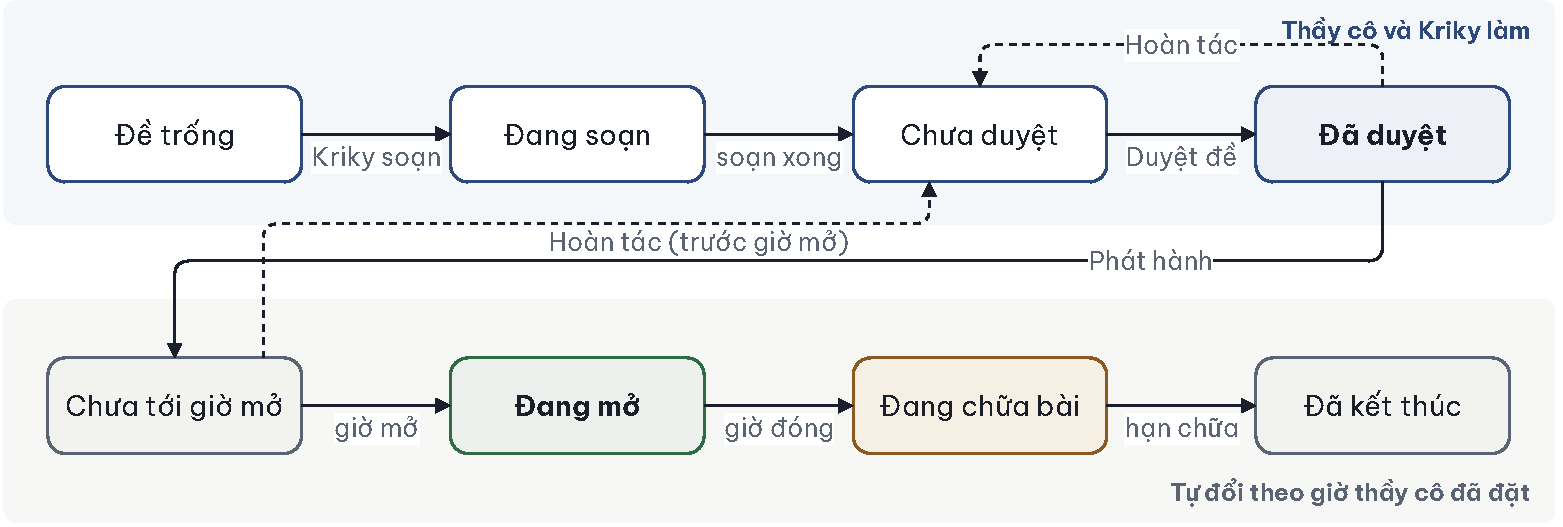
\includegraphics[width=\linewidth]{trang-thai-de.pdf}
  \caption[Trạng thái của một đề]{Trạng thái của một đề. Hàng trên do thầy cô và Kriky làm; hàng dưới
    tự đổi theo giờ thầy cô đã đặt lúc phát hành.}
  \label{fig:trang-thai-de}
\end{figure}

\viec{Duyệt đề}

\anh[0.6\linewidth]{T/19b-duyet-de}{
  \diem{1}{0.2}{0.68}
}

Đọc hết các câu trong khung đề, rồi bấm \nut{Duyệt đề} \sobuoc{1}.

\xong{các câu khoá lại (không còn \nut{Sửa}, \nut{Xoá}), và dưới đề hiện \nhan{Cài đặt phát hành}.}

\machnho{Duyệt đề cũng đưa các câu vào ngân hàng câu hỏi để dùng lại về sau. Duyệt nhầm thì bấm
\nut{Hoàn tác} dưới \nhan{Cài đặt phát hành}: đề về \nhan{Chưa duyệt} và sửa được tiếp.}

\viec{Đặt giờ và phát hành}

\anh[0.62\linewidth]{T/25-cai-dat-phat-hanh}{
  \diem{1}{0.22}{0.145}
  \diem{2}{0.025}{0.32}
  \diem{3}{0.34}{0.32}
  \diem{4}{0.025}{0.42}
  \diem{5}{0.025}{0.6}
  \diem{6}{0.34}{0.6}
  \diem{7}{0.95}{0.65}
  \diem{8}{0.3}{0.93}
}

\begin{buoc}
  \item Bấm lớp sẽ nhận đề (chọn được nhiều lớp).
  \item \nhan{Làm bài}: số phút cho mỗi em làm bài.
  \item \nhan{Mở lúc}: từ giờ này các em bắt đầu làm được.
  \item \nhan{Đóng lúc}: sau giờ này không em nào bắt đầu làm được nữa.
  \item \nhan{Phút mỗi câu}: thời gian cho mỗi câu khi các em làm lại câu sai.
  \item \nhan{Hạn chữa xong}: sau giờ này các em thôi chữa bài.
  \item Đọc khung vàng: Kriky đọc lại các giờ bằng lời để thầy cô kiểm.
  \item Bấm \nut{Phát hành đề}.
\end{buoc}

\begin{bangtra}{L{4.4cm}Y}{\dau{Giờ} & \dau{Cần đúng thế này}}
  \nhan{Mở lúc} & Ở tương lai, sau giờ bấm phát hành. \\
  \nhan{Đóng lúc} & Sau giờ mở. Em vào lúc sát giờ đóng vẫn được làm đủ số phút. \\
  \nhan{Hạn chữa xong} & Sau giờ đóng cộng thời gian làm bài. \\
\end{bangtra}

\viec{Xác nhận phát hành}

\anh[0.62\linewidth]{T/26-xac-nhan-phat-hanh}{
  \diem{1}{0.955}{0.855}
}

Hộp \nhan{Phát hành đề kiểm tra?} đọc lại đề, lớp, giờ và hạn. Đúng hết thì bấm \nut{Phát hành cho 23 học
sinh} \sobuoc{1}. Cần đổi thì bấm \nut{Xem lại cài đặt}.

\xong{khung đề ghi \nhan{ĐÃ PHÁT HÀNH}, thẻ trong chat ghi \nhan{Đã phát hành}.}

\viec{Thu đề về trước giờ mở}

\anh[0.62\linewidth]{T/27-da-phat-hanh}{
  \diem{3}{0.36}{0.9}
}

Phát hành nhầm, hay cần sửa đề, thì thu đề về \textbf{trước giờ mở}:

\begin{buoc}
  \item Mở lại đề: ở \nhan{Các bài kiểm tra} bấm \nut{Mở đoạn chat}, hoặc bấm đoạn chat ấy ở thanh trái
        rồi bấm thẻ đề.
  \item Chỉ thấy dòng \nhan{Cài đặt phát hành} thì bấm vào để mở phần ấy ra.
  \item Bấm \nut{Hoàn tác}.
\end{buoc}

Đề được thu về khỏi mọi lớp và trở lại \nhan{Chưa duyệt}; thầy cô sửa rồi duyệt, phát hành lại.

\luuy{Từ giờ mở, các em đã có thể vào làm, nên không thu đề về được nữa. Chỉ cần một lớp đã tới giờ
mở là \nut{Hoàn tác} khoá. Hoàn tác thu đề khỏi \textbf{mọi} lớp cùng lúc, chưa thu riêng một lớp được.}

\viec{Phát hành thêm cho lớp khác}

Đề đã phát hành vẫn phát thêm được cho lớp chưa nhận: mở khung đề, bấm lớp mới trong \nhan{Cài đặt phát
hành}, đặt giờ, rồi bấm \nut{Phát hành đề}. Lớp đã nhận đề thì chip của nó khoá lại.

\machnho{Ô giờ có thể hiện kiểu 12 giờ, ví dụ \nhan{04:10 CH}: \nhan{CH} là buổi chiều, tức 16:10.}

\machnho{Bỏ dở biểu mẫu giữa chừng thì lần sau mở lại, dòng \nhan{Bản nháp bạn gõ …} giữ các giờ đã gõ.
Bấm \nut{Bỏ bản nháp} để gõ lại từ đầu.}

\chapter{Theo dõi kết quả}
\label{chuong:theo-doi}

Sau giờ mở, thầy cô xem được ai đã nộp, điểm của từng em, câu nào cả lớp sai nhiều và em nào thấy lời
giải thích của Kriky còn khó hiểu.

\viec{Bảng theo dõi}

\anh{T/28-bang-theo-doi}{
  \diem{1}{0.835}{0.284}
  \diem{2}{0.86}{0.36}
}

Bấm \nut{Bảng theo dõi} ở thanh trái. Bảng gom những việc cần thầy cô xem:

\begin{bangtra}{L{3.8cm}L{3cm}Y}{\dau{Loại} & \dau{Bấm} & \dau{Nghĩa là}}
  \nhan{Giải thích chưa rõ} & \sobuoc{1} \nut{Xem báo cáo} & Có em bấm báo Kriky giải thích khó hiểu. \\
  \nhan{Tỉ lệ sai cao} & \sobuoc{2} \nut{Xem câu} & Một câu có từ 70\% bài sai ở lần làm đầu, khi đề có trên 20 bài
  nộp (cộng các lớp). Chỉ hiện sau hạn chữa bài ở mọi lớp. \\
\end{bangtra}

Phần \nhan{Điểm gộp theo lớp} có số khi một đề đã qua hạn chữa bài ở lớp ấy. Điểm ở đây quy về thang
10.

\viec{Xem câu cả lớp sai nhiều}

\anh{T/29-cau-sai-nhieu}{
  \diem{1}{0.07}{0.885}
  \diem{2}{0.26}{0.885}
}

Màn này cho thấy mỗi phương án được bao nhiêu phần trăm học sinh chọn ở lần làm đầu, và lỗi gắn với
phương án sai. Ở ảnh, 77\% chọn \nhan{B. Cực tiểu}: phần lớn lớp nhầm chiều đổi dấu.

\begin{buoc}
  \item Xem xong bấm \nut{Đánh dấu đã xem} để câu rời khỏi bảng theo dõi.
  \item Câu có vấn đề thì bấm \nut{Chỉnh sửa trong Ngân hàng câu hỏi}.
\end{buoc}

\viec{Đọc báo cáo của học sinh}

Ở \nhan{Bảng theo dõi}, bấm \nut{Xem báo cáo} cạnh dòng \nhan{Giải thích chưa rõ}.

\anh{T/30-bao-cao}{
  \diem{1}{0.35}{0.55}
  \diem{3}{0.25}{0.92}
}

\anh[0.62\linewidth]{T/30b-bao-cao-hoc-sinh}{
  \diem{2}{0.4}{0.82}
}

\begin{buoc}
  \item Bên trái là các câu bị báo cáo. Câu cần sửa thì bấm \nut{Chỉnh sửa trong Ngân hàng câu hỏi ›}.
  \item Bên phải là từng báo cáo: em nào, sai câu nào. Bấm \nut{Mở hội thoại hỏi trợ lý ›} để đọc em
        đã hỏi Kriky những gì.
  \item Đọc xong bấm \nut{Đánh dấu đã xem}.
\end{buoc}

\anh[0.8\linewidth]{T/31-hoi-thoai-cua-em}{}

Hộp \nhan{Hội thoại hỏi trợ lý — …} chỉ để đọc. Bấm \nut{Đóng} khi xong.

\viec{Xem kết quả một đề}

\anh{T/32-cac-bai-kiem-tra}{
  \diem{1}{0.845}{0.84}
}

Ở \nhan{Các bài kiểm tra}, đề đã tới giờ mở có \nut{Xem kết quả} \sobuoc{1}. Đề phát hành cho nhiều lớp thì nút này
mở lớp đầu tiên; lớp khác mở từ màn của lớp ấy (Chương~\ref{chuong:lop}).

\anh{T/33-ket-qua-de}{
  \diem{1}{0.81}{0.11}
  \diem{2}{0.21}{0.7}
}

\begin{buoc}
  \item Bấm \nut{Xuất bảng điểm (.xlsx)} để tải bảng điểm về.
  \item Bấm tên một em để xem bài làm của em ấy.
\end{buoc}

\viec{Xem bài làm một em}

\anh{T/34-bai-lam-mot-em}{}

Màn này ghi điểm, số câu đúng ngay lần đầu, số lượt chữa đã làm và số lần em báo giải thích chưa rõ.
Bảng dưới cho thấy từng câu em chọn gì, đáp án là gì, được bao nhiêu điểm.

\viec{Hỏi Kriky về kết quả}

Thầy cô cũng hỏi Kriky được bằng lời trong một đoạn chat. Kriky trả lời số bài đã nộp, điểm trung
bình và số câu còn chữa, ví dụ khi hỏi:

\begin{loinhan}
Lớp 12A làm đề Kiểm tra 15 phút thế nào?
\end{loinhan}

Muốn biết câu nào cả lớp sai nhiều, xem mục \nhan{Tỉ lệ sai cao} của bảng theo dõi.

\chapter{Ngân hàng câu hỏi}

Mỗi lần thầy cô duyệt một đề, các câu của đề ấy vào ngân hàng câu hỏi. Thầy cô dùng lại chúng cho đề sau
(Chương~\ref{chuong:soan-de}, mục \emph{Thêm câu từ ngân hàng}).

\viec{Xem ngân hàng}

\anh{T/35-ngan-hang}{}

Bấm \nut{Ngân hàng câu hỏi} ở thanh trái. Mỗi hàng là một câu, kèm mục kiến thức và khối, môn.

\viec{Sửa một câu trong ngân hàng}

\anh[0.45\linewidth]{T/36-sua-ngan-hang}{}

\begin{buoc}
  \item Bấm vào câu cần sửa. Khung \nhan{Sửa câu trong ngân hàng} mở bên phải.
  \item Sửa \nhan{Đề bài}, \nhan{Phương án} hay \nhan{Cách giải}, rồi bấm \nut{Lưu}.
\end{buoc}

\luuy{Chỉ bản trong ngân hàng thay đổi. Đề đã phát hành vẫn giữ câu cũ; đề sau lấy câu này sẽ dùng bản
mới.}

\chapter{Khi gặp trục trặc}

\begin{bangtra}{L{6.4cm}Y}{\dau{Thầy cô thấy} & \dau{Làm gì}}
  \nhan{Máy này không mở đăng ký. Hãy nhờ người quản trị tạo tài khoản.} & Nhờ người quản lý Kriky của
  trường cấp tài khoản. \\
  \nhan{Bạn nhập sai quá nhiều lần. Thử lại sau N phút.} & Đợi đúng số phút ấy rồi đăng nhập lại. \\
  \nhan{Kriky chưa trả lời kịp. Chữ bạn gõ vẫn còn ở ô nhập.} & Bấm \nut{Gửi} lại. \\
  \nhan{Kriky chưa trả lời được lúc này. Bạn thử gửi lại sau một chút nhé.} & Đợi một lát, gõ lại lời
  nhắn rồi gửi. \\
  Kriky hỏi đi hỏi lại về một cuốn sách & Mở \nut{Đoạn chat mới}, đừng kéo sách vào, ghi rõ \go{không dùng
  tài liệu}. \\
  Tài liệu còn \nhan{Đang đọc …/… trang…} lâu & Số trang đọc được còn tăng thì cứ đợi; sách scan dày cần
  vài phút. Đứng yên lâu thì app tự báo lỗi. \\
  \nhan{Xử lí lỗi. Hãy tải lại} & Tải lại tệp ấy. \\
  Một câu ghi \nhan{Chưa soạn được} & Bấm \nut{Thử lại} trên câu ấy trong khung đề. \\
  \nhan{Công thức có ký tự hỏng…} khi sửa câu & Gõ lại công thức, hoặc nhờ Kriky viết lại. \\
  \nhan{Phương án B chưa có nhãn lỗi…} & Ghi lỗi cho mọi phương án sai ở ô \nhan{Lỗi của …}. \\
  Nút \nut{Phát hành đề} bị khoá & Kiểm đã chọn lớp và điền đủ năm ô giờ; đọc dòng đỏ ngay trên nút nếu
  có. \\
  Phát hành báo giờ mở đã qua & Đặt lại \nhan{Mở lúc} vào tương lai rồi bấm lại. \\
  Phát hành nhầm & Trước giờ mở: bấm \nut{Hoàn tác} (Chương~\ref{chuong:duyet}). Sau giờ mở thì không thu
  về được. \\
  Không thấy nút \nut{Hoàn tác} & Bấm dòng \nhan{Cài đặt phát hành} ở khung đề để mở phần ấy ra. \\
  Học sinh quên mật khẩu & \nut{Đặt lại mật khẩu} ở màn của lớp, rồi đưa em mật khẩu mới. \\
  Đóng hộp mật khẩu mà chưa lưu & Đặt lại mật khẩu cho từng em cần. \\
  Màn hình không cập nhật & Tải lại trang (F5). \\
\end{bangtra}

Khi báo lỗi cho người quản lý Kriky, gửi kèm tên bản ở góc trái dưới màn hình (bấm vào để chép) và một
ảnh chụp màn hình.


% Phần II: học sinh. Chương 10–14 nối số với Phần I.

\trangphan{hs}{Phần II}{Dành cho học sinh}{Đăng nhập, làm bài, hỏi Kriky những câu em làm sai rồi làm
lại để gỡ điểm.}{\item Đăng nhập \item Làm bài \item Xem kết quả và hỏi Kriky \item Làm lại câu sai
\item Khi gặp trục trặc}

\chapter{Đăng nhập}
\label{chuong:dang-nhap-hs}

Em mở địa chỉ trang học sinh: \diachihocsinh. Tên đăng nhập và mật khẩu do thầy cô phát cho em.

\viec{Đăng nhập}

\anh[0.6\linewidth]{S/01-dang-nhap}{
  \diem{1}{0.035}{0.38}
  \diem{2}{0.035}{0.64}
  \diem{3}{0.035}{0.84}
}

\begin{buoc}
  \item Gõ \nhan{Tên đăng nhập} thầy cô phát, ví dụ \go{khangtm}.
  \item Gõ \nhan{Mật khẩu}.
  \item Bấm \nut{Đăng nhập}.
\end{buoc}

\xong{em thấy trang \nhan{Bài của tôi}, góc phải có tên, lớp và mã của em.}

\luuy{Quên mật khẩu thì nhờ thầy cô đặt lại. Em chưa tự đổi mật khẩu được.}

\machnho{Làm bài trên máy dùng chung thì bấm \nut{Đăng xuất} ở góc phải khi xong.}

\chapter{Làm bài}
\label{chuong:lam-bai}

\viec{Tìm bài cần làm}

\anh{S/02-bai-cua-toi}{
  \diem{1}{0.6}{0.81}
  \diem{2}{0.85}{0.81}
}

Mỗi bài ghi môn, số câu, thời gian làm, hạn vào làm và hạn chữa. Nhãn \sobuoc{1} cho biết em làm được gì;
nút \sobuoc{2} là việc em làm tiếp.

\begin{bangtra}{L{4.6cm}Y}{\dau{Nhãn} & \dau{Nghĩa là}}
  \nhan{Chưa tới giờ mở} & Chưa làm được. Đợi tới giờ thầy cô mở. \\
  \nhan{Đang mở} & Bấm \nut{Bắt đầu} để làm. \\
  \nhan{Đang làm} & Em đã bắt đầu; bấm \nut{Tiếp tục}. \\
  \nhan{Cần làm lại 2 câu} & Em còn câu sai gỡ điểm được (Chương~\ref{chuong:lam-lai}). Nếu chỉ có nút
  \nut{Xem kết quả} thì đã qua hạn làm lại. \\
  \nhan{Đã hoàn thành} & Đã xong hết. Bấm \nut{Xem kết quả}. \\
  \nhan{Hết hạn làm lại} & Đã qua hạn chữa. Vẫn xem được kết quả. \\
  \nhan{Đã đóng} & Đã qua giờ đóng mà em chưa làm. \\
\end{bangtra}

\viec{Bắt đầu làm bài}

\anh[0.5\linewidth]{S/03-bat-dau}{}

Bấm \nut{Bắt đầu}, đọc hộp \nhan{Bắt đầu làm bài?} rồi bấm \nut{Bắt đầu làm bài}. Chưa sẵn sàng thì bấm
\nut{Để sau}.

\luuy{Đồng hồ không dừng được, kể cả khi em đóng trang.}

\viec{Chọn đáp án}

\anh{S/04-lam-bai}{
  \diem{1}{0.015}{0.62}
}

\anh[0.5\linewidth]{S/04b-dong-ho}{
  \diem{2}{0.035}{0.12}
  \diem{3}{0.035}{0.45}
  \diem{4}{0.035}{0.83}
}

\begin{buoc}
  \item Bấm vào phương án em chọn. Đổi ý thì bấm phương án khác.
  \item Theo dõi đồng hồ \nhan{Còn lại}.
  \item Bấm các ô số để sang câu khác. Ô đậm là câu đang xem, ô xanh nhạt là câu đã trả lời, ô xám là câu
        chưa làm. Dòng \nhan{CÒN 3 CÂU CHƯA TRẢ LỜI} đếm số câu còn bỏ trống.
  \item Làm xong thì bấm \nut{Nộp bài}.
\end{buoc}

\viec{Nộp bài}

\anh[0.6\linewidth]{S/05-nop-bai}{}

Hộp \nhan{Nộp bài?} đếm lại số câu đã trả lời. Còn câu chưa làm thì bấm \nut{Quay lại làm tiếp}; xong rồi
thì bấm \nut{Nộp bài}.

\luuy{Nộp rồi thì không sửa được nữa. Câu bỏ trống tính là sai.}

\luuy{Đồng hồ về \nhan{00:00} thì em không chọn thêm được nữa. Bấm \nut{Nộp bài} ngay: bài lần đầu
\textbf{không tự nộp}, và chưa nộp thì chưa có kết quả, chưa chữa được.}

\chapter{Xem kết quả và hỏi Kriky}
\label{chuong:hoi-kriky}

Nộp bài xong, em thấy ngay kết quả. Câu sai chưa phải là hết: em hỏi Kriky cho hiểu, rồi làm một câu
tương tự để gỡ điểm. Hình~\ref{fig:vong-chua-bai} là vòng ấy.

\begin{figure}[htbp]
  \centering
  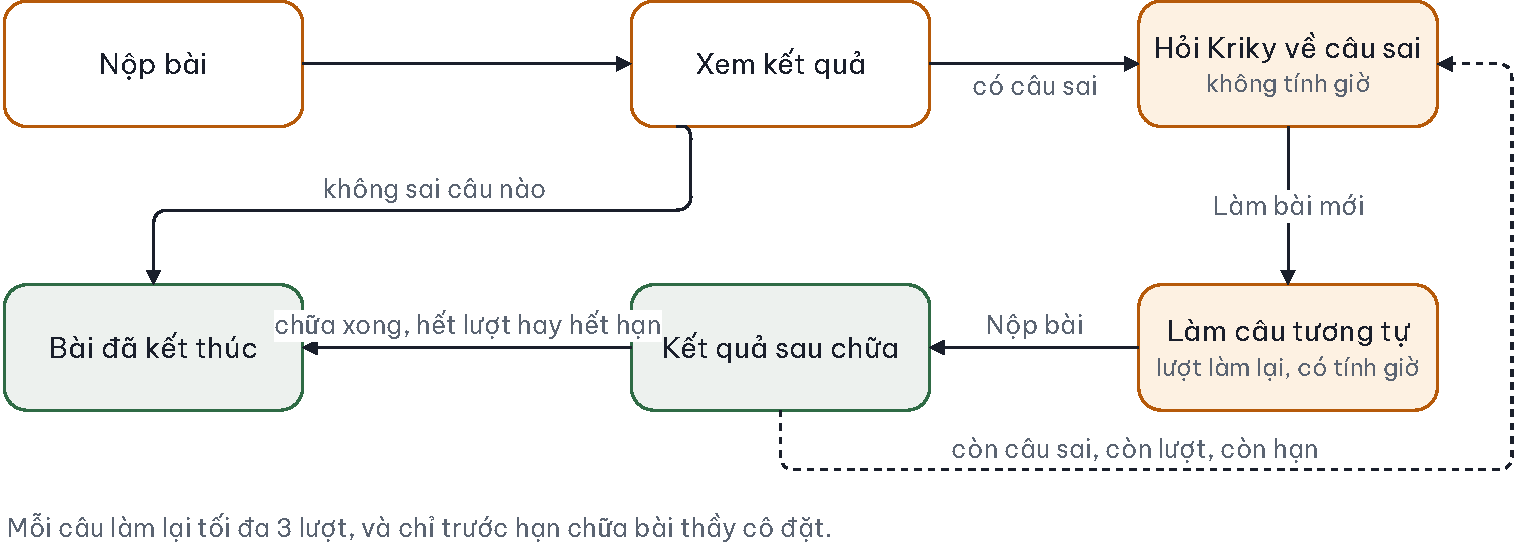
\includegraphics[width=0.9\linewidth]{vong-chua-bai.pdf}
  \caption[Vòng chữa bài]{Vòng chữa bài: hỏi Kriky, làm câu tương tự, tới khi đúng hoặc hết lượt.}
  \label{fig:vong-chua-bai}
\end{figure}

\viec{Xem kết quả}

\anh{S/06-ket-qua}{
  \diem{1}{0.9}{0.86}
  \diem{2}{0.67}{0.09}
}

\begin{buoc}
  \item Câu có vòng tròn rỗng và số 0 bên phải là câu sai; chấm xanh đặc là câu đúng.
  \item Bấm \nut{Hỏi trợ lý và làm lại dạng bài sai} để chữa các câu sai.
\end{buoc}

\machnho{Điểm lúc nộp là điểm sàn. Chữa đúng câu sai trước hạn thì điểm còn tăng.}

\viec{Hỏi Kriky}

\anh[0.6\linewidth]{S/07-hoi-kriky}{}

Gõ câu hỏi vào ô \nhan{Hỏi Kriky về bất kỳ câu nào bạn làm sai…} rồi bấm \nut{Gửi}. Hỏi bằng lời bình
thường, ví dụ:

\begin{loinhan}
Vì sao câu 3 là cực đại mà không phải cực tiểu ạ?
\end{loinhan}

Phần hỏi Kriky không tính giờ. Hỏi tới khi hiểu rồi hãy làm bài mới.

\anh[0.62\linewidth]{S/07b-cau-sai}{
  \diem{1}{0.42}{0.52}
}

Cột bên phải liệt kê \nhan{CÁC CÂU EM LÀM SAI}: em đã chọn gì, đáp án đúng là gì. Bấm \nut{Xem lời giải
đầy đủ ›} \sobuoc{1} để đọc lời giải.

\anh[0.8\linewidth]{S/08-loi-giai}{}

Hộp lời giải có các cách giải và \nhan{ĐỐI CHIẾU TỪNG PHƯƠNG ÁN}: vì sao mỗi phương án đúng hay sai. Bấm
\nut{Đóng} khi xong.

\viec{Báo khi Kriky giải thích khó hiểu}

Khi Kriky đã trả lời câu hỏi đầu tiên của em, nút \nut{Báo cáo Trợ lý giải thích khó hiểu} hiện dưới ô
nhắn. Bấm nút ấy nếu em vẫn chưa hiểu; thầy cô sẽ thấy báo cáo của em.

\anh[0.62\linewidth]{S/09-bao-cao}{}

\xong{nút đổi thành \nhan{Đã báo cho giáo viên}.}

\chapter{Làm lại câu sai}
\label{chuong:lam-lai}

\viec{Bắt đầu lượt làm lại}

\anh[0.6\linewidth]{S/10-bat-dau-lam-lai}{
  \diem{1}{0.972}{0.853}
}

Ở trang hỏi Kriky, bấm \nut{Làm bài mới · 2 câu · 4 phút} (số câu, số phút đổi theo bài). Đọc hộp
\nhan{Bắt đầu lượt làm lại?} (hộp gọi mỗi lượt là một \emph{vòng}) rồi bấm \nut{Làm bài mới} \sobuoc{1}.

Lỡ đóng trang khi đang làm lượt làm lại thì vào lại trang hỏi Kriky: nút đổi thành \nut{Làm tiếp lượt
đang mở}.

\luuy{Bấm là đồng hồ chạy ngay. Gần tới hạn làm lại thì lượt có thể bị dừng giữa chừng.}

\viec{Làm và nộp lượt làm lại}

\anh{S/11-lam-lai}{}

Mỗi câu sai được thay bằng một câu cùng dạng. Em làm như lúc làm bài: chọn đáp án, bấm ô số để sang câu
khác (ô số mang số câu gốc, ví dụ 3 và 6), rồi bấm \nut{Nộp bài}.

\anh[0.6\linewidth]{S/11b-nop-luot}{}

Hộp \nhan{Nộp lượt này?} hỏi lại một lần. Bấm \nut{Nộp bài} để nộp.

\machnho{Hết giờ mà em chưa nộp thì lượt làm lại tự nộp (đã đóng trang thì lượt nộp khi em mở lại).
Câu bỏ trống tính là sai.}

\viec{Xem kết quả sau khi chữa}

\anh{S/12-ket-qua-sau-chua}{}

Câu đã chữa ghi \nhan{Lượt làm lại} và điểm mới. Làm đúng câu tương tự thì câu ấy được 0,5 điểm (nửa
điểm), không phải 1.

\begin{bangtra}{L{5.2cm}Y}{\dau{Em thấy} & \dau{Nghĩa là}}
  Lượt làm lại sai, còn lượt và còn hạn & Hỏi Kriky thêm rồi bấm \nut{Làm bài mới} lần nữa. \\
  Rê chuột lên điểm của câu thấy \nhan{Đã dùng hết ba lượt làm lại cho câu này.} & Câu ấy không chữa
  được nữa. \\
  Bài ghi \nhan{Bài đã kết thúc} & Hết hạn, đã chữa xong hoặc hết lượt. Bấm \nut{Xem lại phần chữa các câu
  sai} để đọc lại. \\
\end{bangtra}

\chapter{Khi gặp trục trặc}

\begin{bangtra}{L{6cm}Y}{\dau{Em thấy} & \dau{Làm gì}}
  Không đăng nhập được & Kiểm tra lại tên đăng nhập, mật khẩu. Vẫn không được thì nhờ thầy cô đặt lại
  mật khẩu. \\
  Không thấy bài thầy cô nói & Hỏi thầy cô bài đã phát hành cho lớp em chưa, hay thầy cô đã thu bài
  về. \\
  \nhan{Bạn nhập sai quá nhiều lần. Thử lại sau N phút.} & Đợi đủ số phút rồi đăng nhập lại. \\
  \nhan{Chưa tới giờ mở} & Đợi tới giờ mở rồi tải lại trang. \\
  Lỡ đóng trang khi đang làm bài & Mở lại trang, bấm \nut{Tiếp tục}. Đồng hồ vẫn chạy trong lúc ấy. \\
  Lỡ đóng trang khi đang làm lượt làm lại & Vào trang hỏi Kriky, bấm \nut{Làm tiếp lượt đang mở}. \\
  Đồng hồ về \nhan{00:00}, bài vẫn \nhan{Đang làm} & Bấm \nut{Nộp bài}. Bài lần đầu không tự nộp. \\
  \nhan{Lượt chữa vừa rồi đã hết giờ nên được nộp luôn…} & Lượt làm lại hết giờ. Câu bỏ trống tính là
  sai; còn lượt thì làm lại. \\
  Nút \nut{Gửi} hỏi Kriky bị khoá & Bài đã kết thúc; em vẫn đọc lại được phần chữa. \\
  Màn hình không cập nhật & Tải lại trang (F5). \\
\end{bangtra}


% Cuối sách: tra nhanh nhãn trạng thái. Không đánh số.

\phanchung
\chapter*{Tra nhanh}
\phantomsection\addcontentsline{toc}{part}{Tra nhanh}

\section{Trạng thái của đề (giáo viên thấy)}

\begin{bangtra}{L{4.2cm}Y}{\dau{Nhãn} & \dau{Nghĩa là}}
  \nhan{Đề trống} & Đề vừa tạo, chưa có câu nào. \\
  \nhan{Đang soạn} & Kriky đang soạn câu. \\
  \nhan{Chưa duyệt} & Có câu, thầy cô chưa duyệt. Sửa, xoá câu được. \\
  \nhan{Đã duyệt} & Đã duyệt, chưa phát hành. Câu đã vào ngân hàng. \\
  \nhan{Chưa tới giờ mở} & Đã phát hành, học sinh chưa làm được. Còn \nut{Hoàn tác} được nếu chưa lớp
  nào tới giờ mở. \\
  \nhan{Đang mở} & Học sinh đang làm bài. \\
  \nhan{Đang chữa bài} & Qua giờ đóng, học sinh đang chữa câu sai. \\
  \nhan{Đã kết thúc} & Qua hạn chữa. Điểm đã chốt. \\
\end{bangtra}

\section{Trạng thái của bài (học sinh thấy)}

Xem bảng ở Chương~\ref{chuong:lam-bai}, mục \emph{Tìm bài cần làm}.

\section{Trạng thái của tài liệu}

Xem bảng ở Chương~\ref{chuong:tai-lieu}, mục \emph{Đọc trạng thái của tài liệu}.

\needspace{0.35\textheight}
\section{Màu trên màn hình}

\begin{bangtra}{L{4.2cm}Y}{\dau{Màu} & \dau{Nghĩa là}}
  \leavevmode\textcolor{correct}{\vua Xanh lá} & Câu đúng. \\
  \leavevmode\textcolor{incorrect}{\vua Đỏ} & Câu sai, hoặc một việc bị lỗi (dải báo lỗi). Chữ đi kèm cho
  biết là cái nào. \\
  \leavevmode\textcolor{needshuman}{\vua Nâu vàng} & Cần người ra tay: một việc chờ thầy cô, hay một tài
  liệu đọc hỏng. \\
  \leavevmode\textcolor{processing}{\vua Xanh ngọc} & Việc của Kriky (đang làm hay vừa xong), đề đang
  mở. \\
  \leavevmode\textcolor{accent}{\vua Xanh dương} & Nút bấm và đường dẫn. \\
\end{bangtra}


\end{document}
